\documentclass[a4paper]{article}
\usepackage[utf8]{inputenc}
\usepackage{geometry}
\usepackage{xcolor}
\geometry{legalpaper, margin=1in}
\usepackage[T1]{fontenc}
\usepackage{algorithm}
\newcommand\tab[1][1cm]{\hspace*{#1}}
\usepackage{graphicx}
\usepackage{listings}

\lstdefinestyle{customc}{belowcaptionskip=1\baselineskip,
breaklines=true,
frame=L,
xleftmargin=\parindent,
language=C,
showstringspaces=false,
basicstyle=\footnotesize\ttfamily,
keywordstyle=\bfseries\color{green!40!black},
commentstyle=\itshape\color{purple!40!black},
identifierstyle=\color{blue},
stringstyle=\color{orange},
}

\lstset{literate=
  {á}{{\'a}}1 {é}{{\'e}}1 {í}{{\'i}}1 {ó}{{\'o}}1 {ú}{{\'u}}1
  {Á}{{\'A}}1 {É}{{\'E}}1 {Í}{{\'I}}1 {Ó}{{\'O}}1 {Ú}{{\'U}}1
  {à}{{\`a}}1 {è}{{\`e}}1 {ì}{{\`i}}1 {ò}{{\`o}}1 {ù}{{\`u}}1
  {À}{{\`A}}1 {È}{{\'E}}1 {Ì}{{\`I}}1 {Ò}{{\`O}}1 {Ù}{{\`U}}1
  {ä}{{\"a}}1 {ë}{{\"e}}1 {ï}{{\"i}}1 {ö}{{\"o}}1 {ü}{{\"u}}1
  {Ä}{{\"A}}1 {Ë}{{\"E}}1 {Ï}{{\"I}}1 {Ö}{{\"O}}1 {Ü}{{\"U}}1
  {â}{{\^a}}1 {ê}{{\^e}}1 {î}{{\^i}}1 {ô}{{\^o}}1 {û}{{\^u}}1
  {Â}{{\^A}}1 {Ê}{{\^E}}1 {Î}{{\^I}}1 {Ô}{{\^O}}1 {Û}{{\^U}}1
  {œ}{{\oe}}1 {Œ}{{\OE}}1 {æ}{{\ae}}1 {Æ}{{\AE}}1 {ß}{{\ss}}1
  {ű}{{\H{u}}}1 {Ű}{{\H{U}}}1 {ő}{{\H{o}}}1 {Ő}{{\H{O}}}1
  {ç}{{\c c}}1 {Ç}{{\c C}}1 {ø}{{\o}}1 {å}{{\r a}}1 {Å}{{\r A}}1
  {€}{{\euro}}1 {£}{{\pounds}}1 {«}{{\guillemotleft}}1
  {»}{{\guillemotright}}1 {ñ}{{\~n}}1 {Ñ}{{\~N}}1 {¿}{{?`}}1
}
\lstset{escapechar=@,style=customc,tabsize=3}

\title{SDD : TP 3}
\author{Mathieu Boutin - Jérémy Morceaux}
\begin{document}
\maketitle
\section{Présentation générale}
- Ce TP a pour but de travailler sur la représentation des arbres en mémoire. Tout d'abord, il fallait créer un arbre en utilisant la représentation lien vertical/horizontal. Puis de vérifier le résultat avec le débuggeur ddd. Ensuite, il fallait afficher cette arbre avec la représentation postfixée. Par la suite, il fallait créer une méthode d'insertion dans l'arbre. Il fallait également créer un autre type d'arbre où chaque noeud possède l'arbre du noeud père à partir de l'arbre de base. Finalement, il fallait afficher la représentation postfixée de ce nouvel arbre.
\\
\\
\underline{- Schéma de base :}
\begin{center}
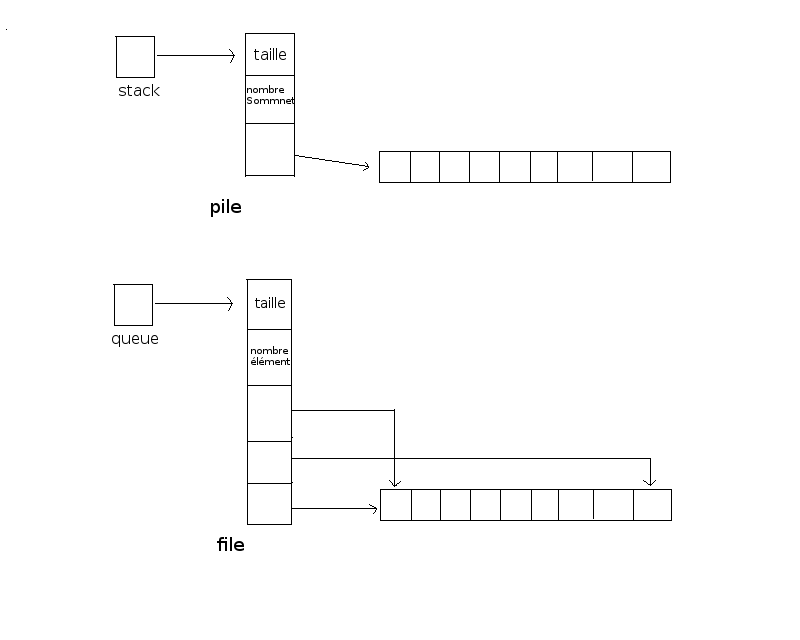
\includegraphics[scale=0.4]{Schema_base.png}
\\
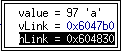
\includegraphics[scale=1]{structure_arbre_base.png}
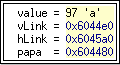
\includegraphics[scale=1]{structure_arbre_modifie.png}
\\
noeud de l'arbre de base / noeud de l'arbre générée à partir de l'arbre de base
\end{center}
\underline{Vérification avec DDD :}

\begin{center}
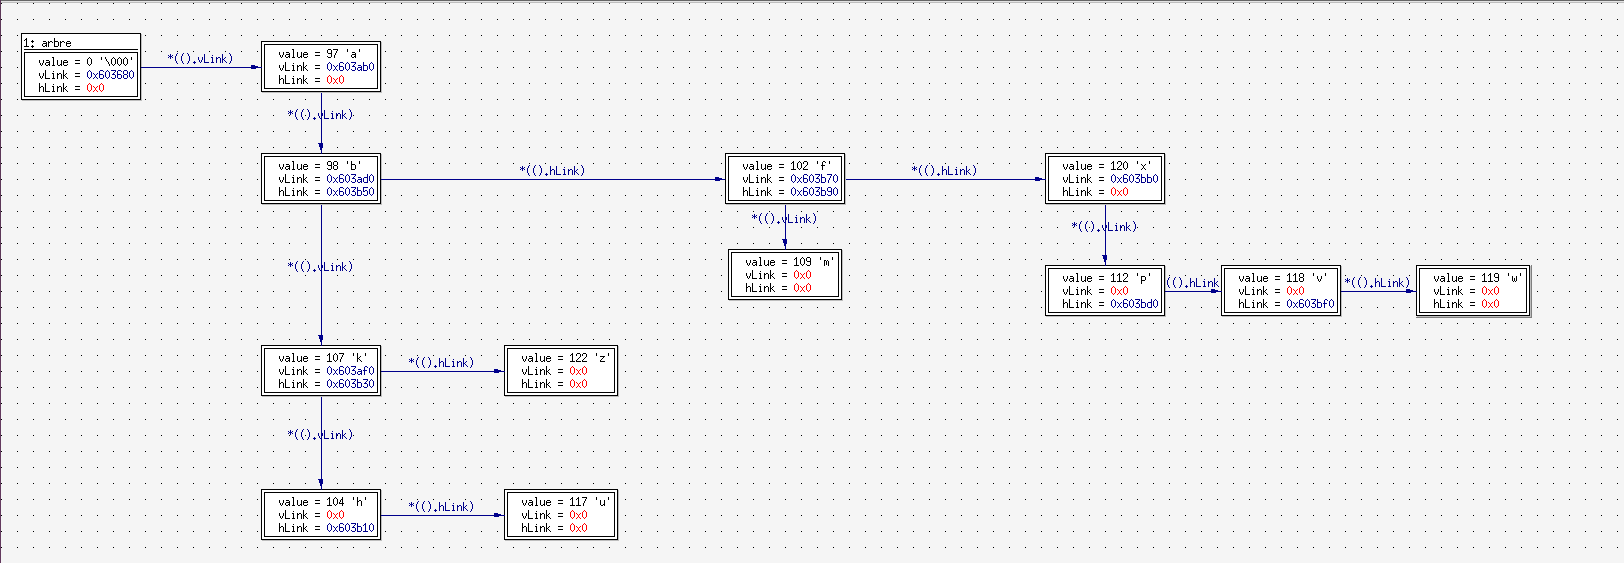
\includegraphics[scale=0.2]{image_arbre_base.png}

Arbre de base obtenu grâce à DDD
\end{center}

\begin{center}
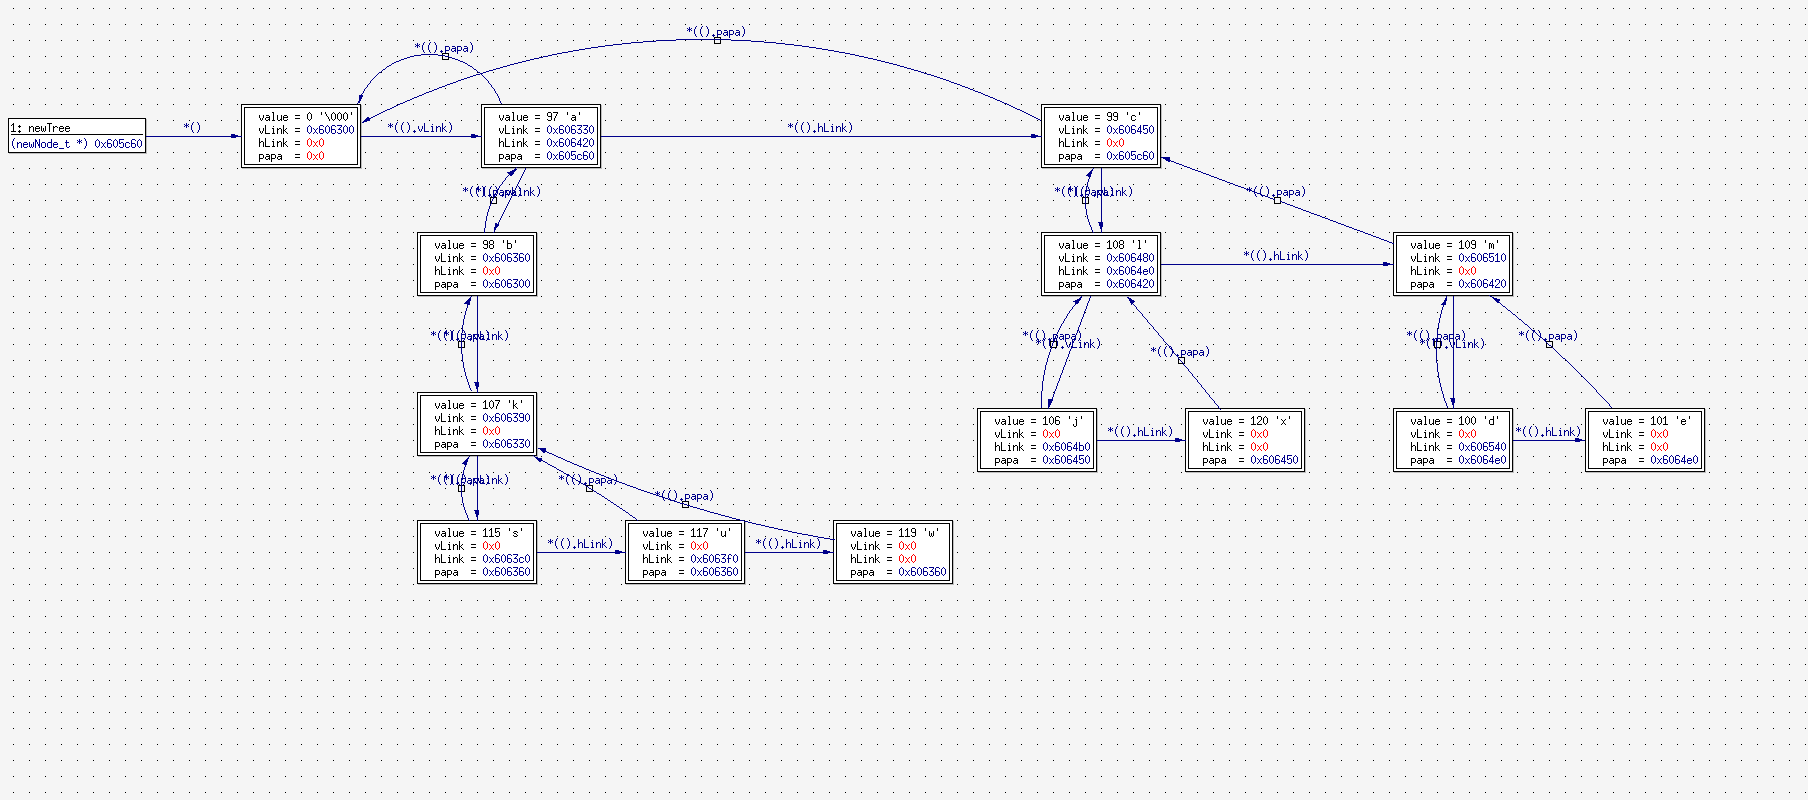
\includegraphics[scale=0.2]{foret_newNode.png}

Arbre avec lien vers le père obtenu grâce à DDD
\end{center}

\section{Détail de chaque fonction}

\subsection{main}
\begin{algorithm}
Principe : main
\\
\\
\tab On crée un arbre à partir de la chaîne de caractère treeString.
\\
\tab Si la création a réussi:
\\
\tab \tab Si l'arbre est non-vide:
\\
\tab \tab \tab On affiche la représentation postfixée.
\\
\tab \tab \tab On recherche le noeud sur lequel on veut insérer le nouveau noeud.
\\
\tab \tab \tab Si on a trouvé le noeud.
\\
\tab \tab \tab \tab On insère celui-ci dans l'arbre
\\
\tab \tab \tab \tab Si l'insertion a réussi:
\\
\tab \tab \tab \tab \tab On affiche un message de compliment.
\\
\tab \tab \tab \tab Sinon
\\
\tab \tab \tab \tab \tab On affiche un message d'erreur.
\\
\tab \tab \tab On affiche la représentation postfixée du nouvel arbre.
\\
\tab \tab \tab On crée un nouvel arbre à partir de l'arbre de base.
\\
\tab \tab \tab Si la création a réussi:
\\
\tab \tab \tab \tab On affiche la représentation postfixée de ce nouvel arbre.
\\
\tab \tab \tab Sinon
\\
\tab \tab \tab \tab On affiche un message d'erreur.
\\
\tab \tab \tab On libére l'arbre de base.
\\
\tab \tab \tab On libère l'arbre généré à partir de l'arbre de base.
\\
\tab \tab Sinon
\\
\tab \tab \tab On affiche un message d'erreur.
\\
\tab Sinon
\\
\tab \tab on affiche un message d'erreur
\\
\tab On libère la tête de l'arbre de base
\\
FIN
\end{algorithm}
\underline{Lexique :}
\begin{itemize}
\item Variables locales:
\begin{itemize}
\item arbre: c'est le pointeur vers l'arbre de base.
\item errorCode: indique si une fonction s'est bien déroulée.
\item treeString: chaine de caractère permettant la création de l'arbre de base.
\item pere: pointeur vers le noeud du père du noeud à insérer.
\item newtree: pointeur vers l'arbre généré à partir de l'arbre de base.
\item p: caractère du père pour le nouveau noeud à insérer
\item i: caractère du noeud à insérer
\end{itemize}
\end{itemize}
\underline{Programme Commenté :}

\lstinputlisting[language=C, firstline=1, lastline=134]{main.c}

\subsection{createNode}

\begin{algorithm}
Principe :  createNode (char courant)
\\
\\
\tab on alloue un nouveau noeud
\\
\tab On lui associe courant comme valeur
\\
\tab On fait pointer vers NULL ses autres pointeurs
\\
\tab On renvoie le noeud
\\
FIN
\end{algorithm}
\underline{Lexique :}
\begin{itemize}
\item Paramètre(s) de la fonction  
\begin{itemize}
\item courant : caractère associé au nouveau noeud.
\end{itemize}
\item Variables locales:
\begin{itemize}
\item node : contient la structure de nouveau noeud qui sera renvoyé.
\end{itemize}
\end{itemize}
\underline{Programme Commenté :}

\lstinputlisting[language=C, firstline=25, lastline=38]{ZZ_tree.c}

\newpage
\subsection{incrementNbSon}

\begin{algorithm}
Principe :  incrementNbSon
\\
\\
\tab on recupère le dernier élément empiler dans stack
\\
\tab on ajoute +1 à son nombre de fils
\\
\tab on remet cet élément dans la pile
\\
FIN
\end{algorithm}
\underline{Lexique :}
\begin{itemize}
\item Paramètre(s) de la fonction  
\begin{itemize}
\item stack : c'est la pile qui contient des noeuds de l'arbre.
\item elmt : permet de recupérer un noeud de la pile.
\item errorCode : indique si l'opération (pop ou push) s'est bien déroulée
\end{itemize}
\end{itemize}
\underline{Programme Commenté :}

\lstinputlisting[language=C, firstline=51, lastline=61]{ZZ_tree.c}


\subsection{pushBis}
\begin{algorithm}
Principe : pushBis
\\
\\
\tab On initialise notre nouvel élément
\\
\tab On met son nombre de fils à 1
\\
\tab On met cet élément dans la pile
\\
FIN
\end{algorithm}
\underline{Lexique :}
\begin{itemize}
\item Paramètre(s) de la fonction  
\begin{itemize}
\item stack : c'est la pile qui contient des noeuds de l'arbre.
\item elmt : permet de recupérer un noeud de la pile.
\item errorCode : indique si l'opération (pop ou push) s'est bien déroulée.
\item cur : c'est le noeud que l'on veut empiler.
\end{itemize}
\end{itemize}
\underline{Programme Commenté :}

\lstinputlisting[language=C, firstline=74, lastline=81]{ZZ_tree.c}

\newpage
\subsection{repPostFixe}
\begin{algorithm}
Principe : repPostFixe
\\
\\
\tab On initialise des pointeurs, une pile et des variables;
\\
\tab Si l'arbre est non vide alors:
\\
\tab \tab Tant qu'on n'a pas parcouru tout l'arbre faire:
\\
\tab \tab \tab Si l'élément a déjà été traité alors :
\\
\tab \tab \tab \tab On affiche l'élément avec son nombre de fils;
\\
\tab \tab \tab \tab S'il a un frère alors:
\\
\tab \tab \tab \tab \tab On accède à son frère;
\\
\tab \tab \tab \tab Sinon: 
\\
\tab \tab \tab \tab \tab On accède à son père s'il en a un;
\\
\tab \tab \tab Sinon: [S'il n'a pas déjà été traité]
\\
\tab \tab \tab \tab Tant qu'il existe un fils faire :
\\
\tab \tab \tab \tab \tab On accède au fils de l'élément;
\\
\tab \tab \tab \tab On affiche le dernier fils;
\\
\tab \tab \tab \tab S'il a un frère alors:
\\
\tab \tab \tab \tab \tab On accède à son frère;
\\
\tab \tab \tab \tab Sinon: [il n'a pas de frère]
\\
\tab \tab \tab \tab \tab On accède à son père si il existe;
\\
FIN
\end{algorithm}
\underline{Lexique :}
\begin{itemize}
\item Paramètre(s) de la fonction  
\begin{itemize}
\item L'adresse de l'arbre
\item L'adresse d'une variable de Code Erreur
\end{itemize}
\item Variables locales:
\begin{itemize}
\item cur est le pointeur courant qui parcourt l'arbre
\item stack est la pile qui servira à stocker les élément lors du parcours et de remonter dans l'arbre
\item elmt  est le type d'élément stocké dans la pile stack 
\item wasInStack est un entier représentant un booléen afin de savoir si l'élément a déjà été empilé et donc traité
\item end est un entier traduisant un booléen afin de savoir si on a parcouru tout l'arbre 
\end{itemize}
\end{itemize}
\underline{Programme Commenté :}

\lstinputlisting[language=C, firstline=93, lastline=225]{ZZ_tree.c}

\subsection{createTree}
\begin{algorithm}
Principe : createTree
\\
\\
\tab On initialise une pile, des pointeurs de parcours, et des variables
\\
\tab Pour chaque caractère de notre chaine :
\\
\tab \tab Si le caractère courant est une parenthèse ouvrante:
\\
\tab \tab \tab On le sauvegarde pour la prochaine itération
\\
\tab \tab Si le caractère est une parenthèse fermante :
\\
\tab \tab \tab Si la pile est non vide:
\\
\tab \tab \tab \tab On la dépile pour faire pointer le noeud de parcours sur un noeud père
\\
\tab \tab \tab Sinon:
\\
\tab \tab \tab \tab On s'arrête
\\
\tab \tab Si le caractère est une virgule:
\\
\tab \tab \tab On le sauvegarde pour la prochaine itération
\\
\tab \tab Sinon [Si c'est une lettre]:
\\
\tab \tab \tab On ajoute un noeud au noeud courant : sur le le lien vertical si le caracètre pécèdent 
\\
\tab \tab \tab était une parenthèse ouvrante, sur le lien horizontale si le caractère précèdent était une
\\
\tab \tab \tab virgule ou une parenthèse fermante.
\\
\tab On renvoie l'arbre
\\
\tab Si il y a eu un problème lors de la création
\\
\tab \tab On libère l'arbre !
\\
\\
FIN
\end{algorithm}
\underline{Lexique :}
\begin{itemize}
\item Paramètre(s) de la fonction  
\begin{itemize}
\item treeString contient la chaîne de caractère décrivant l'arbre à créer.
\end{itemize}
\item Variable(s) locale(s)
\begin{itemize}
\item curr est le pointeur courant qui parcourt la liste.
\end{itemize}
\end{itemize}
\underline{Programme commenté :}

\lstinputlisting[language=C, firstline=237, lastline=360]{ZZ_tree.c}

\subsection{rechercher}
\begin{algorithm}
Principe : rechercher
\\
\\
\tab On initialise des pointeurs et des variables;
\\
\tab Si l'arbre est non Vide alors:
\\
\tab \tab Tant qu'on a pas parcouru tout l'arbre ou qu'on n'a pas trouvé la valeur v faire:
\\
\tab \tab \tab Si l'élément a un fils alors:
\\
\tab \tab \tab \tab On stock l'élément dans la file;
\\
\tab \tab \tab Si l'élément possède un frère alors:
\\
\tab \tab \tab \tab on accède à son frère;
\\
\tab \tab \tab Sinon:
\\
\tab \tab \tab \tab Si la file est non vide alors:
\\
\tab \tab \tab \tab \tab On retourne sur le premier élément enfilé;
\\
\tab \tab \tab \tab Sinon:
\\
\tab \tab \tab \tab \tab On a parcouru tout l'arbre, on s'arrête;
\\
FIN
\end{algorithm}
\underline{Lexique :}
\begin{itemize}
\item Paramètre(s) de la fonction  
\begin{itemize}
\item L'adresse de l'arbre
\item L'adresse d'une variable de Code Erreur
\item La valeur v du nœud à chercher
\end{itemize}
\item Variables locales:
\begin{itemize}
\item cur est le pointeur courant qui parcourt l'arbre
\item queue est la file qui servira à stocker les élément lors du parcours de l'arbre selon le 1er ordre 
\item end est un entier traduisant booléen
\end{itemize}
\end{itemize}
\underline{Programme Commenté :}

\lstinputlisting[language=C, firstline=373, lastline=452]{ZZ_tree.c}

\subsection{createNodeForInsertion}
\begin{algorithm}
Principe : createNodeForInsertion 
\\
\\
\tab On crée une structure qu'on alloue
\\
\tab On lui associe un caractère w.
\\
\tab On lui associe un lien horizontal
\\
\tab Le reste pointe vers NULL.
\\
\tab On renvoie cette structure.
\\
FIN
\end{algorithm}
\underline{Lexique :}
\begin{itemize}
\item Paramètre(s) de la fonction  
\begin{itemize}
\item w : c'est le caractère associé au nouveau noeud.
\item horizontal : c'est le lien horizontal du nouveau noeud. Il peut-être NULL.
\end{itemize}
\item Variables locales:
\begin{itemize}
\item temp : pointeurs vers la nouvelle structure crée.
\end{itemize}
\end{itemize}
\underline{Programme Commenté :}

\lstinputlisting[language=C, firstline=463, lastline=474]{ZZ_tree.c}

\newpage
\subsection{insertNode}
\begin{algorithm}
Principe : insertNode 
\\
\\
\tab On initialise des pointeurs et des variables;
\\
\tab Si le père existe:
\\
\tab \tab S'il n'a pas de fils alors :
\\
\tab \tab \tab On insère en tête le fils;
\\
\tab \tab Sinon: [il a au moins un fils]
\\
\tab \tab \tab Si le premier fils est avant que le fils à insérer dans l'ordre alphabétique alors:
\\
\tab \tab \tab \tab Tant qu'on n'a pas trouvé la place où on insère le fils faire: 
\\
\tab \tab \tab \tab \tab On parcourt ses frères
\\
\tab \tab \tab \tab Si on est à la fin des fils alors:
\\
\tab \tab \tab \tab \tab On insère le fils à la fin des fils;
\\
\tab \tab \tab \tab Sinon: [on a trouvé une place où insérer le fils entre 2 frères]
\\
\tab \tab \tab \tab \tab Si le fils n'existe pas déjà alors:
\\
\tab \tab \tab \tab \tab \tab On insère le fils;
\\
\tab \tab \tab \tab \tab Sinon: [ le fils existe déjà pas besoin ]
\\ 
\tab \tab \tab \tab \tab \tab On met fin au parcours;
\\ 
\tab \tab \tab Sinon: [alors on l'insère en tête ]
\\
\tab \tab \tab \tab On insère le fils;
\\
FIN
\end{algorithm}
\underline{Lexique :}
\begin{itemize}
\item Paramètre(s) de la fonction  
\begin{itemize}
\item L'adresse du nœud où l'on doit insérer le fils
\item L'adresse d'une variable de Code Erreur
\item La valeur w du fils à insérer
\end{itemize}
\item Variables locales:
\begin{itemize}
\item cur est le pointeur courant qui parcourt l'arbre
\item prec est le pointeur qui pointe sur l'élément précédent, ici sur le frère précédent
\end{itemize}
\end{itemize}
\underline{Programme Commenté :}

\lstinputlisting[language=C, firstline=487, lastline=550]{ZZ_tree.c}

\subsection{createModifiedNode}
\begin{algorithm}
Principe : createModifiedNode
\\
\\
\tab On crée un nouveau noeud modifié.
\\
\tab On lui associe le caractère du noeud curr
\\
\tab Les autres pointeurs sont initialisés à NULL;
\\
\tab La valeur papa du noeud est initialisée à NULL.
\\
\tab On renvoie le nouveau noeud.
\\
FIN
\end{algorithm}
\underline{Lexique :}
\begin{itemize}
\item Paramètre(s) de la fonction  
\begin{itemize}
\item cur : c'est le noeud qui donne la valeur à notre nouveau noeud.
\item pere : le pointeur papa de nouvelle structure pointera vers le noeud pere
\end{itemize}
\item Variables locales:
\begin{itemize}
\item node : c'est le pointeur vers notre nouvelle structure
\end{itemize}
\end{itemize}
\underline{Programme Commenté :}

\lstinputlisting[language=C, firstline=561, lastline=572]{ZZ_tree.c}
\newpage
\subsection{copyTree}
\begin{algorithm}
Principe : copyTree 
\\
\\
\tab On initialise une pile, la tête du nouvel arbre, et des variables de parcours/contrôle.
\\
\tab Si l'arbre est non-vide :
\\
\tab \tab Tant qu'on a pas parcouru l'arbre ou rencontré une erreur:
\\
\tab \tab \tab Tant que le noeud courant possède un lien vertical et que c'est la première fois qu'on le visite
\\
\tab \tab \tab \tab On crée un noeud modifié à partir du noeud courant/
\\
\tab \tab \tab \tab On empile ce noeud dans la pile.
\\
\tab \tab \tab \tab On fait descendre le pointeur courant et le père dans la hiérarchie.
\\
\tab \tab \tab Si le noeud courant possède un frère :
\\
\tab \tab \tab \tab On crée un noeud modifié à partir du noeud courant.
\\
\tab \tab \tab \tab On fait pointer le noeud courant vers son frère.
\\
\tab \tab \tab Sinon
\\
\tab \tab \tab \tab Si la pile est non vide
\\
\tab \tab \tab \tab \tab On récupère le dernier élément de la pile.
\\
\tab \tab \tab \tab \tab On modifie les pointeurs de parcours du nouvel arbre grâce au père du 
\\
\tab \tab \tab \tab \tab noeud courant.
\\ 
\tab \tab \tab \tab Sinon
\\ 
\tab \tab \tab \tab \tab On s'arrête.
\\
\tab On renvoie le nouvel arbre.
\\
FIN
\end{algorithm}
\underline{Lexique :}
\begin{itemize}
\item Paramètre(s) de la fonction  
\begin{itemize}
\item tree : c'est le pointeur de l'arbre que l'on veut copier
\item errorCode : indique si la fonction s'est bien déroulée 
\end{itemize}
\item Variables locales:
\begin{itemize}
\item newTree: c'est le pointeur vers le nouvel arbre.
\item end: contrôle la terminaison de l'algorithme.
\item wasInStack: indique si le noeud courant a déjà été parcouru.
\item cur: est le pointeur courant qui parcourt l'arbre de base.
\item stack: c'est le pointeur de la pile.
\item currNewTree: c'est le pointeur de parcours du nouvel arbre.
\item father : pointeur de parcours qui pointe sur le père du pointeur courant.
\item elmt: variable qui permet d'empiler un noeud dans la pile.
\item errorCodeStack : indique si il y a eu un problème avec la pile.
\end{itemize}
\end{itemize}
\underline{Programme Commenté :}

\lstinputlisting[language=C, firstline=583, lastline=710]{ZZ_tree.c}

\subsection{posFixNotationFather}
\begin{algorithm}
Principe : posFixNotationFather
\\
\\
\tab On initialise une pile et des variables de parcours/contrôle.
\\
\tab Si l'arbre est non-vide :
\\
\tab \tab Tant qu'on a pas parcouru l'arbre ou rencontré une erreur:
\\
\tab \tab \tab Tant que le pointeur courant à un fils et qu'il n'a pas déjà été parcouru
\\
\tab \tab \tab \tab On descend le noeud courant dans l'arbre.
\\
\tab \tab \tab Si le noeud courant n'a pas été déjà visité:
\\
\tab \tab \tab \tab On affiche le noeud courant.
\\
\tab \tab \tab Si le noeud courant possède un frère :
\\
\tab \tab \tab \tab On parcourt via le lien horizontal
\\
\tab \tab \tab Sinon
\\
\tab \tab \tab \tab Tant que le père du noeud courant est non-null ou que le noeud courant a un lien 
\\
\tab \tab \tab \tab horizontal null
\\
\tab \tab \tab \tab \tab On remonte dans l'arbre avec le lien du père.
\\
\tab \tab \tab \tab \tab On affiche le noeud courant.
\\
\tab \tab \tab \tab Si on a atteint la tête de l'arbre.
\\
\tab \tab \tab \tab \tab on s'arrête.
\\
FIN
\end{algorithm}
\underline{Lexique :}
\begin{itemize}
\item Paramètre(s) de la fonction  
\begin{itemize}
\item tree : c'est le pointeur de l'arbre que l'on veut afficher
\end{itemize}
\item Variables locales:
\begin{itemize}
\item cur: est le pointeur courant qui parcourt l'arbre de base.
\item end: contrôle la terminaison de l'algorithme.
\item backFromFather: indique si le noeud courant a déjà été parcouru.
\end{itemize}
\end{itemize}
\underline{Programme Commenté :}

\lstinputlisting[language=C, firstline=720, lastline=778]{ZZ_tree.c}

\subsection{freeTreeFather}
\begin{algorithm}
Principe : freeTreeFather
\\
\\
\tab On initialise des variables de parcours/contrôle.
\\
\tab Si l'arbre est non-vide :
\\
\tab \tab \tab Tant qu'on a pas parcouru tout l'arbre ou rencontré un problème:
\\
\tab \tab \tab \tab Tant que le noeud courant a un fils et qu'il n'a pas déjà été visité
\\
\tab \tab \tab \tab \tab on descend dans la hiérarchie de l'arbre.
\\
\tab \tab \tab \tab Si le noeud courant n'a pas déjà été visité
\\
\tab \tab \tab \tab \tab On enregistre le noeud courant
\\
\tab \tab \tab \tab Si le noeud courant a un frère
\\
\tab \tab \tab \tab \tab Si le noeud a déjà été visité
\\
\tab \tab \tab \tab \tab \tab On enregistre le noeud courant
\\
\tab \tab \tab \tab \tab On parcourt via le lien horizontal
\\
\tab \tab \tab \tab \tab On libère le noeud enregistré
\\
\tab \tab \tab \tab Sinon
\\
\tab \tab \tab \tab Tant que le père du noeud courant n'est pas NULL et que le frère du noeud 
\\
\tab \tab \tab \tab courant est NULL
\\
\tab \tab \tab \tab \tab Si le noeud courant a déjà été visité
\\
\tab \tab \tab \tab \tab \tab On enregistre le noeud courant
\\
\tab \tab \tab \tab \tab On revient en arrière grâce au père du noeud courant
\\
\tab \tab \tab \tab \tab On libère le noeud enregistré
\\
\tab \tab \tab \tab Si on a atteint la tête de l'arbre
\\
\tab \tab \tab \tab \tab On s'arrête.
\\
\tab On libère le noeud enregistré.
\\
FIN
\end{algorithm}
\underline{Lexique :}
\begin{itemize}
\item Paramètre(s) de la fonction  
\begin{itemize}
\item tree : c'est le pointeur de l'arbre que l'on veut libérer
\end{itemize}
\item Variables locales:
\begin{itemize}
\item cur: est le pointeur courant qui parcourt l'arbre.
\item end: contrôle la terminaison de l'algorithme.
\item backFromFather: indique si le noeud courant a déjà été parcouru.
\item temp: cette variable enregistre les noeuds courant à libérer.
\end{itemize}
\end{itemize}
\underline{Programme Commenté :}

\lstinputlisting[language=C, firstline=788, lastline=860]{ZZ_tree.c}
\newpage
\subsection{freeTree}
\begin{algorithm}
Principe : freeTree
\\
\\
\tab On initialise une pile et des variables de parcours/contrôle.
\\
\tab Si l'arbre est non-vide :
\\
\tab \tab Si l'élément courant a déjà été parcouru:
\\
\tab \tab \tab Tant qu'on a pas parcouru tout l'arbre ou rencontré un problème:
\\
\tab \tab \tab \tab On enregistre le noeud courant.
\\
\tab \tab \tab \tab Si le noeud courant possède un frère:
\\
\tab \tab \tab \tab \tab On parcours via le lien horizontal
\\
\tab \tab \tab \tab Sinon
\\
\tab \tab \tab \tab \tab Si la pile est non vide:
\\
\tab \tab \tab \tab \tab \tab On récupère le dernier élément empilé.
\\
\tab \tab \tab \tab \tab Sinon :
\\
\tab \tab \tab \tab \tab \tab On s'arrête.
\\
\tab \tab Sinon:
\\
\tab \tab \tab Tant que le noeud courant a un fils:
\\
\tab \tab \tab \tab on empile le noeud courant.
\\
\tab \tab \tab \tab On passe à son fils.
\\
\tab \tab \tab On enregistre le noeud courant.
\\
\tab \tab \tab Si le noeud courant a un frère:
\\
\tab \tab \tab \tab On parcourt via le lien horizontal.
\\
\tab \tab \tab Sinon:
\\
\tab \tab \tab \tab Si la pile est non-vide:
\\
\tab \tab \tab \tab \tab on récupère le dernier élément empilé.
\\
\tab \tab \tab \tab Sinon:
\\
\tab \tab \tab \tab \tab On s'arrête.
\\
\tab \tab \tab On libère le noeud enregistré.
\\
\tab On libère la pile.
\\
FIN
\end{algorithm}
\underline{Lexique :}
\begin{itemize}
\item Paramètre(s) de la fonction  
\begin{itemize}
\item tree : c'est le pointeur de l'arbre que l'on veut libérer
\end{itemize}
\item Variables locales:
\begin{itemize}
\item cur: est le pointeur courant qui parcourt l'arbre.
\item stack: pile contenant des noeuds de l'arbre à supprimer.
\item elmt: variable qui permet d'empiler des noeuds.
\item end: contrôle la terminaison de l'algorithme.
\item wasInStack: indique si le noeud courant a déjà été parcouru.
\item errorCodeStack: indique si il y a eu un problème avec la pile.
\end{itemize}
\end{itemize}
\underline{Programme Commenté :}

\lstinputlisting[language=C, firstline=870, lastline=995]{ZZ_tree.c}

\section{Compte rendu d'exécution}

\subsection{Cas : Cas général}
treeString = (a(b(k(h,u)z)f(m)x(p,v,w)))
\\ 
SIZE\_STACK = 50
\\
noeud d'insertion = b
\\
noeud à insérer = l
\\
\\
\underline{Sortie: }
\begin{center}
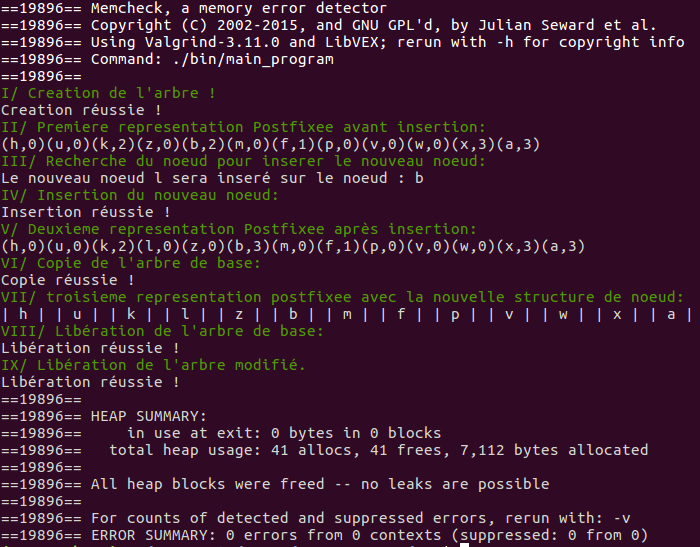
\includegraphics[scale=0.6]{cas_general.png}
\\
Cas général
\end{center}

\subsection{Cas : 2 forêts}
treeString = (a(b(k(u,w)))c(l(j,x)m(d,e)))
\\ 
SIZE\_STACK = 50
\\
noeud d'insertion = a
\\
noeud à insérer = l
\\
\\
\underline{Sortie: }
\begin{center}
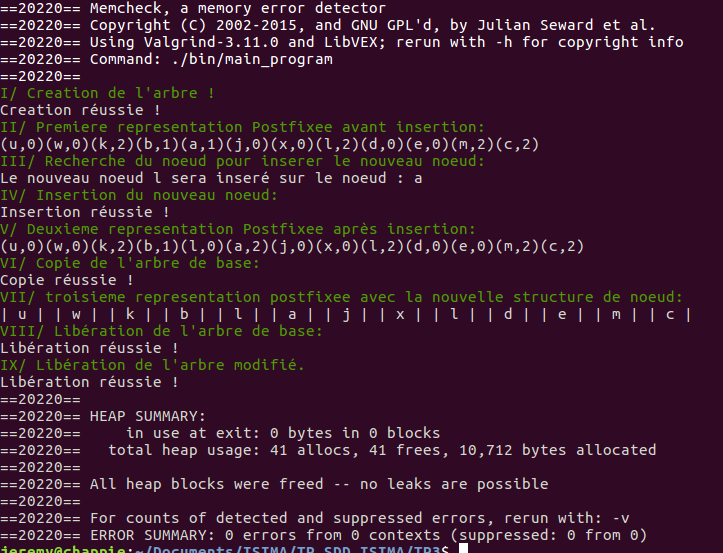
\includegraphics[scale=0.6]{2foret.png}
\\
2 forêts
\end{center}

\subsection{Cas : Arbre vertical}
treeString = (a(b(k)))
\\ 
SIZE\_STACK = 50
\\
noeud d'insertion = a
\\
noeud à insérer = l
\\
\\
\underline{Sortie: }
\begin{center}
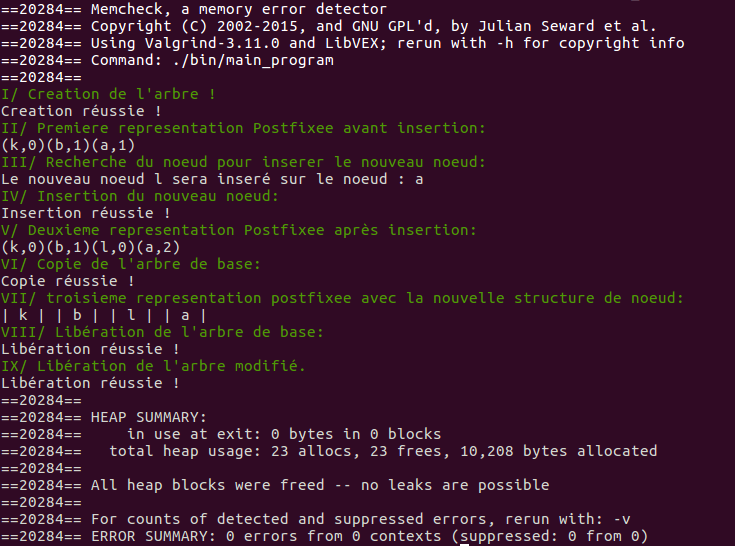
\includegraphics[scale=0.6]{vertical.png}
\\
Arbre Vertical
\end{center}

\subsection{Cas : Arbre horizontal}
treeString = (a,b,c)
\\ 
SIZE\_STACK = 50
\\
noeud d'insertion = a
\\
noeud à insérer = l
\\
\\
\underline{Sortie: }
\begin{center}
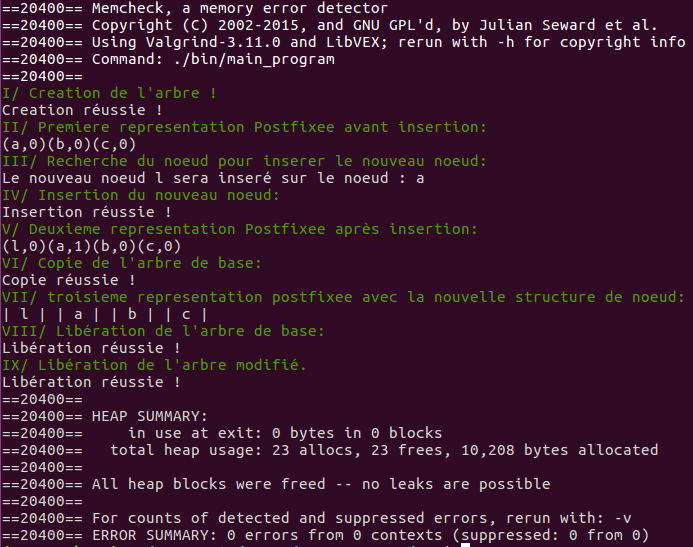
\includegraphics[scale=0.6]{horizontal.png}
\\
Arbre horizontal
\end{center}

\subsection{Cas : Le noeud d'insertion n'existe pas}
treeString = (a(b(k(h,u)z)f(m)x(p,v,w)))
\\ 
SIZE\_STACK = 50
\\
noeud d'insertion = g
\\
noeud à insérer = l
\\
\\
\underline{Sortie: }
\begin{center}
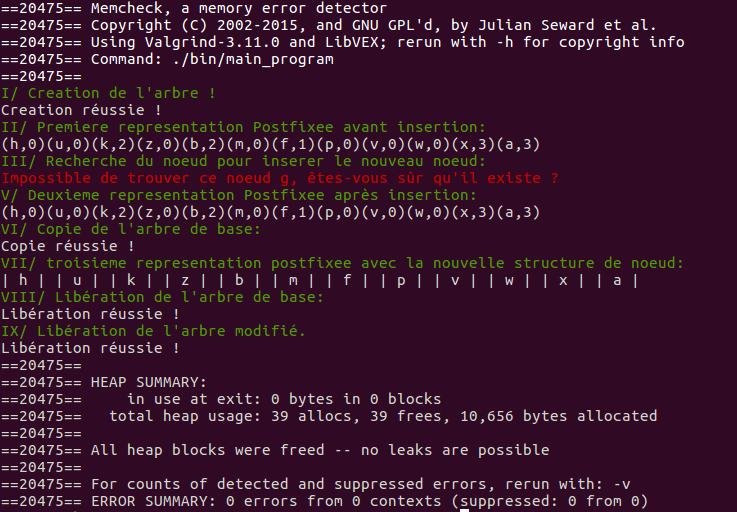
\includegraphics[scale=0.6]{pere_existe_pas.png}
\\
Le noeud d'insertion n'existe pas
\end{center}

\subsection{Cas : Insertion du noeud sur la tête de l'arbre}
treeString = (a(b(k(h,u)z)f(m)x(p,v,w)))
\\ 
SIZE\_STACK = 50
\\
noeud d'insertion = ! \underline{( le caractère '!' est reservée pour  identifier la tête )}
\\
noeud à insérer = l
\\
\\
\underline{Sortie: }
\begin{center}
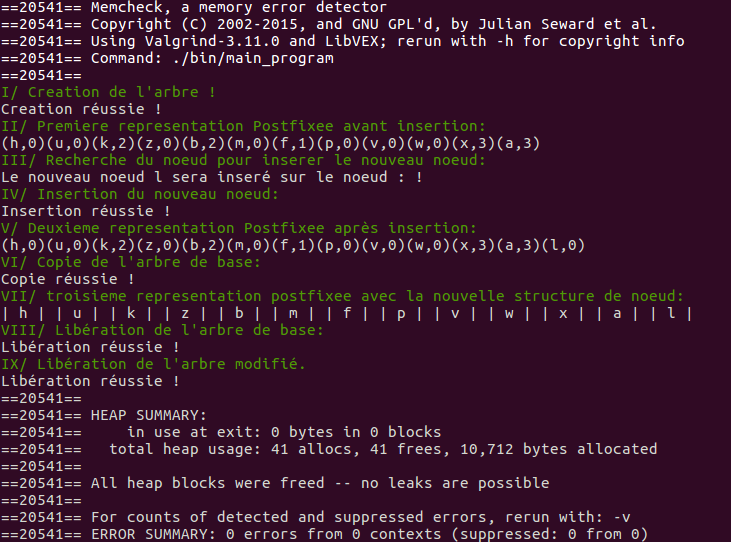
\includegraphics[scale=0.6]{insertion_tete.png}
\\
Insertion du noeud sur la tête de l'arbre
\end{center}

\subsection{Cas : Arbre vide}
treeString = ()
\\ 
SIZE\_STACK = 50
\\
noeud d'insertion = a
\\
noeud à insérer = l
\\
\\
\underline{Sortie: }
\begin{center}
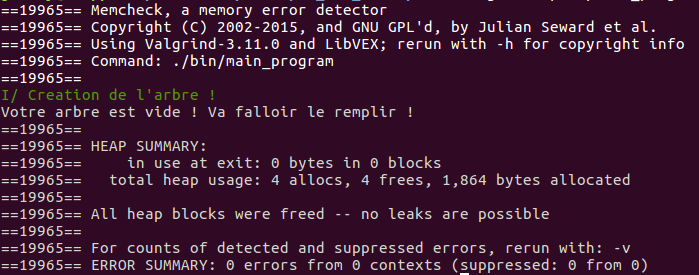
\includegraphics[scale=0.6]{vide.png}
\\
Arbre vide
\end{center}

\subsection{Cas : Le noeud est déjà présent sur le noeud père}
treeString = (a(b(k(h,u)z)f(m)x(p,v,w)))
\\ 
SIZE\_STACK = 50
\\
noeud d'insertion = k
\\
noeud à insérer = h
\\
\\
\underline{Sortie: }
\begin{center}
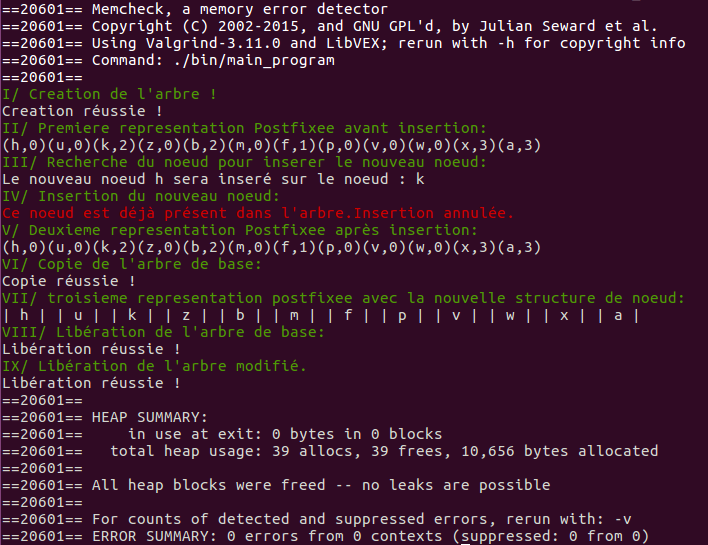
\includegraphics[scale=0.6]{noeud_present.png}
\\
Le noeud est déjà présent sur le noeud père
\end{center}

\subsection{Cas : Stack de taille 2}
treeString = (a(b(k(h,u)z)f(m)x(p,v,w)))
\\ 
SIZE\_STACK = 2
\\
noeud d'insertion = b
\\
noeud à insérer = l
\\
\\
\underline{Sortie: }
\begin{center}
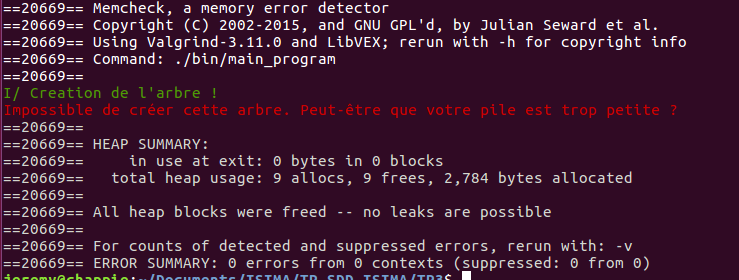
\includegraphics[scale=0.6]{stack_2.png}
\\
Stack de taille 2
\end{center}

\subsection{Cas : Stack de taille 0}
treeString = (a(b(k(h,u)z)f(m)x(p,v,w)))
\\ 
SIZE\_STACK = 0
\\
noeud d'insertion = b
\\
noeud à insérer = l
\\
\\
\underline{Sortie: }
\begin{center}
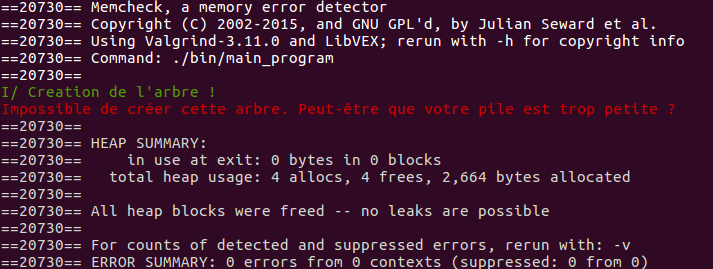
\includegraphics[scale=0.6]{stack_0.png}
\\
Stack de taille 0
\end{center}

\end{document}
